\section{Software Design}

\subsection{Usecase description}

\begin{figure}[htbp]
	\centering
		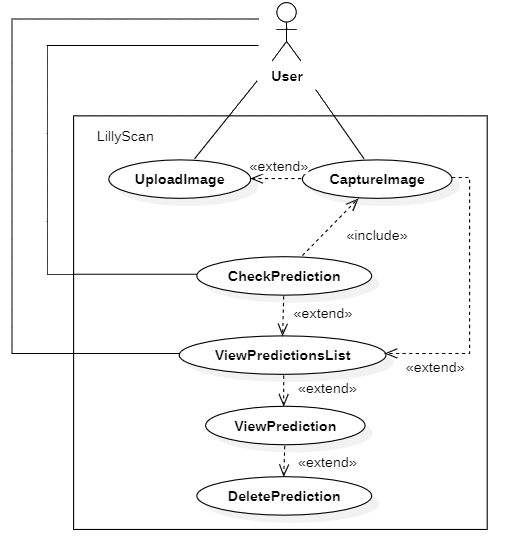
\includegraphics[scale=0.6]{figures/usecase_diagram.png}
	\caption{The use case diagram}	        
\end{figure}

\begin{longtable}{|p{.20\textwidth}|p{.80\textwidth} |}
 \hline
 \textbf{ID and name} & UC01 CaptureImage \\ 
 \hline
 \textbf{Primary actor} & User \\ 
 \hline
 \textbf{Description} & The user makes a photo using the camera. \\ 
 \hline
 \textbf{Trigger} & The user opens the application. \\ 
 \hline
 \textbf{Preconditions} &  \\  
 \hline
 \textbf{Postconditions} & POST-1. The system obtains an image object as an input. \\ 
 \hline
 \textbf{Normal flow} & 
 \textbf{1.0. Take a picture}
 1. The user taps on the application icon. \newline 
 2. The application opens the camera preview screen. \newline
 3. The user clicks on the "Take photo" button. \newline
 4. The system asks the user to confirm their action. \newline
 5. The user validates the picture taken. \newline
 6. The system starts UC3. CheckPrediction. \\ 
 \hline
 \textbf{Alternative flows} & 
 \textbf{1.1. Retake picture} \newline
 Steps 1,\ldots,4 from \textbf{1.0} \newline
 5. The user chooses the retry option. \newline
 6. The system follows the normal flow, starting from step 2. \\ \hline 
\end{longtable}

\begin{longtable}{|p{.20\textwidth}|p{.80\textwidth} |}
 \hline
 \textbf{ID and name} & UC02. UploadImage \\ 
 \hline
 \textbf{Primary actor} & User \\ 
 \hline
 \textbf{Description} & The user loads an image from the filesystem. \\ 
 \hline
 \textbf{Trigger} & The user chooses the "Load picture" option on the camera screen. \\ 
 \hline
 \textbf{Preconditions} &  \\  
 \hline
 \textbf{Postconditions} & POST-1. The system obtains an image object as an input. \\ 
 \hline
 \textbf{Normal flow} & 
 \textbf{1.0. Load picture} \newline
 1. The system opens the file picker dialog. \newline 
 2. The user chooses the target image. \newline
 3. The system starts UC3. CheckPrediction.
 \\ \hline
 \textbf{Alternative flows} & 
\textbf{1.1. Cancel picture loading} \newline
 1. The system opens the file picker dialog. \newline 
 2. The user cancels the file picker dialog. \newline
 3. The system starts UC01. CaptureImage. \\
 \hline 
\end{longtable}

\begin{longtable}{|p{.20\textwidth}|p{.80\textwidth} |}
 \hline
 \textbf{ID and name} & UC03. CheckPredictions \\ 
 \hline
 \textbf{Primary actor} & User \\ 
 \hline
 \textbf{Description} & The system segments the text lines and makes a prediction of the writing \\ 
 \hline
 \textbf{Trigger} & The user confirms the selection of an image. \\ 
 \hline
 \textbf{Preconditions} & PRE-1. The user provides an input image. \\  
 \hline
 \textbf{Postconditions} & POST-1. The system outputs a list of segmented lines and their corresponding predicted text. \\ 
 \hline
 \textbf{Normal flow} & 
 \textbf{1.0. Validate prediction} \newline
 1. The system shows the predicted output. \newline 
 2. The user clicks the "Save record" button. \newline
 3. The system adds the result to the predictions list. \newline
 4. The system starts UC04. CheckPredictionsList.
 \\ \hline
 \textbf{Alternative flows} & 
 \textbf{1.1. Cancel operation} \newline
 1. The system shows the predicted output. \newline 
 2. The user clicks the "Retry" button. \newline
 3. The system starts UC01. CaptureImage.
 \\ \hline 
\end{longtable}

\begin{longtable}{|p{.20\textwidth}|p{.80\textwidth} |}
 \hline
 \textbf{ID and name} & UC04. ViewPredictionsList \\ 
 \hline
 \textbf{Primary actor} & User \\ 
 \hline
 \textbf{Description} & The user can view a list of stored predictions. \\ 
 \hline
 \textbf{Trigger} & The user clicks the list icon on the camera preview screen, or confirms a prediction. \\ 
 \hline
 \textbf{Preconditions} &  \\  
 \hline
 \textbf{Postconditions} & The predictions list is displayed \\ 
 \hline
 \textbf{Normal flow} & \textbf{1.0. Display list} \newline
 1. The system shows the list of prediction.
 \\ \hline
\end{longtable}

\begin{longtable}{|p{.20\textwidth}|p{.80\textwidth} |}
 \hline
 \textbf{ID and name} & UC05. ViewPrediction \\ 
 \hline
 \textbf{Primary actor} & User \\ 
 \hline
 \textbf{Description} & The user views a prediction contents. \\ 
 \hline
 \textbf{Trigger} & The user selects an item from the predictions list. \\ 
 \hline
 \textbf{Preconditions} & The predictions list is not empty. \\
 \hline
 \textbf{Postconditions} & The system shows the prediction data. \\ 
 \hline
 \textbf{Normal flow} & 
  \textbf{1.0. Display prediction} \newline
 1. The user taps on an entry in the prediction list. \newline
 2. The system displays information about the selected prediction.
 \\ \hline
\end{longtable}

\begin{longtable}{|p{.20\textwidth}|p{.80\textwidth} |}
 \hline
 \textbf{ID and name} & UC06. DeletePrediction \\ 
 \hline
 \textbf{Primary actor} & User \\ 
 \hline
 \textbf{Description} & The user removes the selected prediction.\\ 
 \hline
 \textbf{Trigger} & The user taps the "Delete" icon on the prediction view screen \\ 
 \hline
 \textbf{Preconditions} & The user selects an item from the predictions list.  \\  
 \hline
 \textbf{Postconditions} & The selected prediction no longer exists in the list. \\ 
 \hline
 \textbf{Normal flow} & \textbf{1.0. Remove prediction} \newline
1. The user initiates the remove action. \newline
2. The system prompts for confirmation. \newline
3. The user validates the operation. \newline
4. The system removes the selected item from the prediction list. \newline
5. The system starts UC04. ViewPredictionsList. 
 \\ \hline
 \textbf{Alternative flows} & \textbf{1.0. Remove prediction denied} \newline
Steps 1,2 from normal flow. \newline
3. The user cancels the operation. \newline
5. The system starts UC05. ViewPrediction.
 \\ \hline 
\end{longtable}

\subsection{Conceptual model}

The application consists of two main components: the frontend (user interface), and the computation backend, which hosts most of the AI logic. The latter will be discussed in a separate section due to its overwhelming complexity. The frontend follows a Domain-Driven Design (DDD) type of architecture \cite{DDD}. A Prediction class (Figure \ref{FigClassDiagDomRepo}) is responsible with serving an image and the AI processed output data in a way that is easy to diggest by the UI logic, while the heavy computations happen on RawBitmap image type, which, as the name implies, is a data type that provides fast direct pixel access. For memory optimization reasons, the images travelling inside the view system are described by a class ImageRef containing path reference and a prefabricated thumbnail for quick display whenever necessary (e.g. as icons in the predictions list). The real images are obtained only at prediction view time by passing the ImageRef object through an ImageResolver class which retrieves the full picture data from the filesystem.

\begin{figure}[htbp]
	\centering
		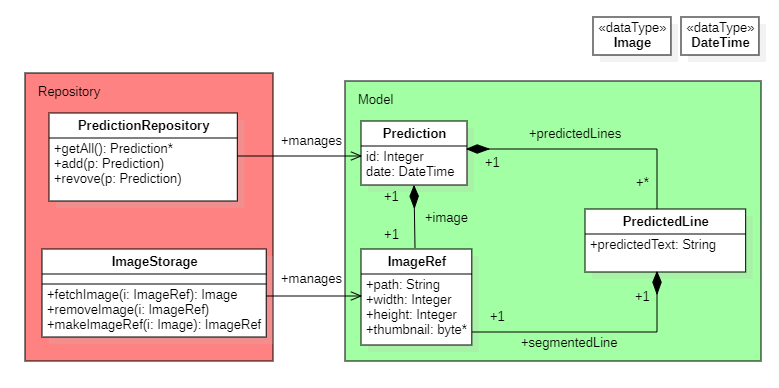
\includegraphics[scale=0.7]{figures/class_diagram_domain_repo.png}
	\caption{Class diagram (domain and repository)}
        \label{FigClassDiagDomRepo}
\end{figure}

\begin{figure}[htbp]
	\centering
		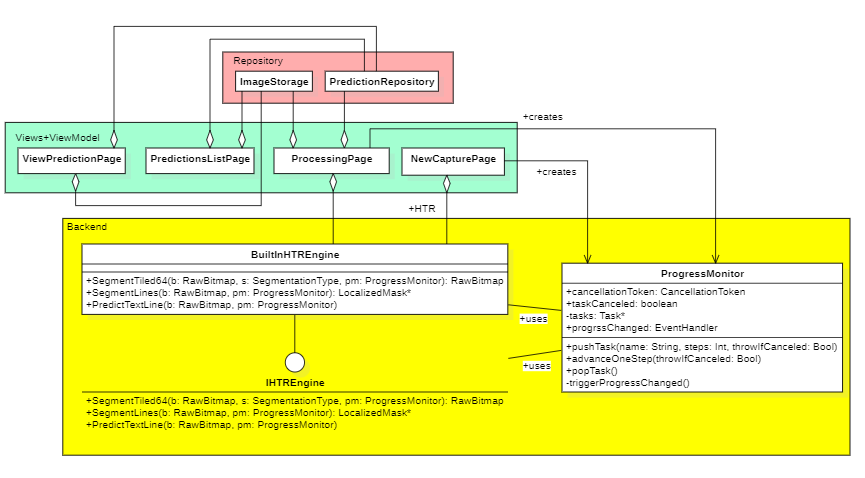
\includegraphics[scale=0.65]{figures/class_diagram_service.png}
	\caption{Class diagram (service and UI)}
        \label{FigClassDiagService}
\end{figure}


 A singleton HTREngine encapsulates segmentation and recognition models, and handles the low level preprocessing and predicting actions (Figure \ref{FigClassDiagService}). These actions are supervised by a ProgressMonitor object which signals the UI the state of a time expensive operation in progress percents. These are used for loading messages and effects in the applications. The ProgressMonitor is also aware of task cancellation, which may trigger either by user request or by environmental factors (e.g. unloading a view or switching page), and handles the phenomenon in a safe fashion.

\subsection{Dynamic model}

\begin{figure}[htbp]
	\centering
		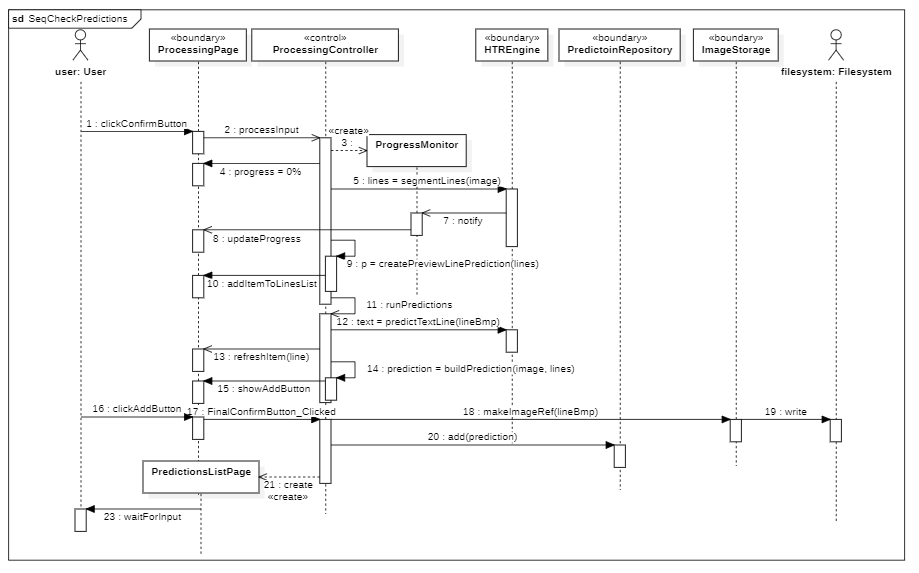
\includegraphics[scale=0.65]{figures/dynamic_model_checkPrediction.PNG}
	\caption{Dynamic model for UC03.CheckPrediction}
        \label{FigDynamicModelCP}
\end{figure}

The application follows a simple linear flow which responds to user interactions. However, since the most recurrent scenario requires waiting for a complex operation to finish, taking additional measures to handle task interruption or cancelation and keeping the user interface responsive may prove to be an interesting challenge. For reference, Figure \ref{FigDynamicModelCP} explains how a ProgressMonitor instance is used to track the progress of an operation and send a completion percentage to the UI. 


